\documentclass[14pt, a4paper]{extarticle}
\usepackage{GOST}
\usepackage{array}
\usepackage{verbatim}
\usepackage[detect-all]{siunitx}
\usepackage{amsmath}
\usepackage{amssymb}
\usepackage[utf8]{inputenc}
\usepackage{hyperref}
\usepackage{tempora}

\makeatletter
\renewcommand\@biblabel[1]{#1.}
\makeatother

\usepackage{listings}
\lstset{ 
	language=C,
	basicstyle=\small, 
	numbers=left, 
	numberstyle=\tiny,
	stepnumber=1,
	numbersep=5pt,
	showspaces=false,            
	showstringspaces=false,      
	showtabs=false,             
	frame=single,            % рисовать рамку вокруг кода
	tabsize=4,      
	commentstyle=\color{green},
	keywordstyle=\color{blue}\textbf,
	numberstyle=\scriptsize\color{gray}, % the style that is used for the line-numbers
	rulecolor=\color{black},
	captionpos=t,
	breaklines=true,         % автоматически переносить строки 
	breakatwhitespace=false, % переносить строки по пробелу
	%escapeinside={\#*}{*)} 
}


\usepackage{pgfplots}
\usepackage{filecontents}
\usetikzlibrary{datavisualization}
\usetikzlibrary{datavisualization.formats.functions}

\begin{document}
	
\begin{table}[ht]
	\centering
	\begin{tabular}{|c|p{400pt}|} 
		\hline
		\begin{tabular}[c]{@{}c@{}} 
\includegraphics[scale=1]{source/b_logo.jpg} \\\end{tabular} &
		\footnotesize\begin{tabular}[c]{@{}c@{}}\textbf{Министерство~науки~и~высшего~образования~Российской~Федерации}\\\textbf{Федеральное~государственное~бюджетное~образовательное~учреждение}\\\textbf{~высшего~образования}\\\textbf{«Московский~государственный~технический~университет}\\\textbf{имени~Н.Э.~Баумана}\\\textbf{(национальный~исследовательский~университет)»}\\\textbf{(МГТУ~им.~Н.Э.~Баумана)}\\\end{tabular}  \\
		\hline
	\end{tabular}
\end{table}
\noindent\rule{\textwidth}{4pt}
\noindent\rule[14pt]{\textwidth}{1pt}
\hfill 
\noindent
\makebox{ФАКУЛЬТЕТ~}%
\makebox[\textwidth][l]{\underline{~«Информатика и системы управления»~~~~~~~~~~~~~~~~~~~~~~~~~~~~~~~~~}}%
\\
\noindent
\makebox{КАФЕДРА~}%
\makebox[\textwidth][l]{\underline{~«Программное обеспечение ЭВМ и информационные технологии»~}}%
\\

\begin{center}
	\vspace{1.5cm}
	{\bf\huge Отчёт\par}
	{\bf\Large по лабораторной работе № 6\par}
	\vspace{0.7cm}
\end{center}


\noindent
\makebox{\large{\bf Название:}~~~}
\makebox[\textwidth][l]{\large\underline{~Реализация монитора Хоара «Читатели-писатели» }}\\
\makebox{\large\underline{~под ОС Windows~}}


\noindent
\makebox{\large{\bf Дисциплина:}~~~}
\makebox[\textwidth][l]{\large\underline{~Операционные системы~~~~~~~~~~~~~~~~~~~~~~~~~~}}\\

\vspace{1.5cm}
\noindent
\begin{tabular}{l c c c c c}
	Студент      & ~ИУ7-55Б~               & \hspace{2.5cm} & \hspace{2cm}                 & &  Д.О. Склифасовский \\\cline{2-2}\cline{4-4} \cline{6-6} 
	\hspace{3cm} & {\footnotesize(Группа)} &                & {\footnotesize(Подпись, дата)} & & {\footnotesize(И.О. Фамилия)}
\end{tabular}

\noindent
\begin{tabular}{l c c c c}
	Преподаватель & \hspace{5cm}   & \hspace{2cm}                 & & ~~~~~~Н.Ю. Рязанова~~~~~~\\\cline{3-3} \cline{5-5} 
	\hspace{3cm}  &                & {\footnotesize(Подпись, дата)} & & {\footnotesize(И.О. Фамилия)}
\end{tabular}

\vspace{0.6cm}
\begin{center}	
	\vfill
	\large \textit {Москва, 2020}
\end{center}

\thispagestyle {empty}
\pagebreak

\clearpage
\section*{Задание}
В лабораторной работе необходимо разработать многопоточное приложение, используя API ОС Windows такие как, потоки, события (event) и мьютексы (mutex). Потоки разделяют единственную глобальную переменную. Приложение реализует монитор Хоара «Читатели-писатели».\par

\textbf{Программа:}
\begin{lstlisting}[label=task1, caption=Задание]
#include <stdio.h>
#include <windows.h>
#include <iostream>

#define WRITERS 3
#define READERS 5
#define MAX_VAL 10

#define OK 0
#define ERROR 1

int value = 0;

bool activeWriter = false;
unsigned int activeReaders = 0;

unsigned int waitingReaders = 0;
unsigned int waitingWriters = 0;

HANDLE writers[WRITERS];
HANDLE readers[READERS];

HANDLE canRead;
HANDLE canWrite;
HANDLE mutex;

void StartRead()
{
	InterlockedIncrement(&waitingReaders);
	if (activeWriter || waitingWriters > 0)
	{
		WaitForSingleObject(canRead, INFINITE);
	}
	InterlockedDecrement(&waitingReaders);
	InterlockedIncrement(&activeReaders);
	SetEvent(canRead);
}

void StopRead()
{
	InterlockedDecrement(&activeReaders);
	if (activeReaders == 0)
	{
		SetEvent(canWrite);
	}
}

void StartWrite()
{
	InterlockedIncrement(&waitingWriters);
	if (activeWriter || activeReaders > 0)
	{
		WaitForSingleObject(canWrite, INFINITE);
	}
	InterlockedDecrement(&waitingWriters);
	activeWriter = true;
}

void StopWrite()
{
	activeWriter = false;
	ResetEvent(canWrite);
	if (waitingWriters)
	{
		SetEvent(canWrite);
	}
	else
	{
		SetEvent(canRead);
	}
}

DWORD WINAPI Reader(LPVOID lpParam)
{
	bool isEnd = FALSE;
	while (!isEnd)
	{
		StartRead();
		
		if (value >= MAX_VAL)
		{
			isEnd = TRUE;
		}
		else
		{
			printf("Reader %d (%d) read %d\n", (int)lpParam, GetCurrentThreadId(), value);
		}
		
		StopRead();
		Sleep(200);
	}
	return OK;
}

DWORD WINAPI Writer(LPVOID lpParam)
{
	bool isEnd = FALSE;
	while (!isEnd)
	{
		StartWrite();
		WaitForSingleObject(mutex, INFINITE);
		
		if (value >= MAX_VAL)
		{
			isEnd = TRUE;
		}
		else
		{
			value++;
			printf("Writer %d (%d) wrote %d\n", (int)lpParam, GetCurrentThreadId(), value);
		}
		
		ReleaseMutex(mutex);
		StopWrite();
		Sleep(200);
	}
	return OK;
}

bool CheckHandle(HANDLE cur, const char* msg)
{
	if (cur == NULL)
	{
		CloseHandle(mutex);
		CloseHandle(canRead);
		CloseHandle(canWrite);
		perror(msg);
		return false;
	}
	return true;
}

int CreateThreads() 
{
	for (int i = 0; i < WRITERS; i++)
	{
		writers[i] = CreateThread(NULL, 0, &Writer, (LPVOID)i, 0, NULL);
		if (!CheckHandle(writers[i], "Thread"))
		{
			return ERROR;
		}
	}
	
	for (int i = 0; i < READERS; i++)
	{
		readers[i] = CreateThread(NULL, 0, &Reader, (LPVOID)i, 0, NULL);
		if (!CheckHandle(readers[i], "Thread"))
		{
			return ERROR;
		}
	}
	
	return OK;
}

int InitHandles()
{
	mutex = CreateMutex(NULL, FALSE, NULL);
	if (mutex == NULL)
	{
		perror("mutex");
		return ERROR;
	}
	
	canRead = CreateEvent(NULL, FALSE, FALSE, TEXT("ReadEvent"));
	if (canRead == NULL)
	{
		CloseHandle(mutex);
		perror("canRead");
		return ERROR;
	}
	
	canWrite = CreateEvent(NULL, TRUE, FALSE, TEXT("WriteEvent"));
	if (canWrite == NULL)
	{
		CloseHandle(mutex);
		CloseHandle(canRead);
		perror("canWrite");
		return ERROR;
	}
	
	return OK;
}

int main() 
{
	if (InitHandles() == ERROR || CreateThreads() == ERROR)
	{
		return ERROR;
	}
	
	WaitForMultipleObjects(WRITERS, writers, TRUE, INFINITE);
	WaitForMultipleObjects(READERS, readers, TRUE, INFINITE);
	
	CloseHandle(mutex);
	CloseHandle(canRead);
	CloseHandle(canWrite);
	
	return 0;
}
\end{lstlisting}

\textbf{Результат работы программы:}\par
\begin{figure}[h!]
	\centering
	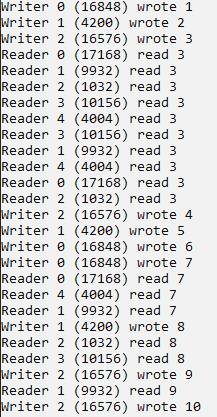
\includegraphics[scale=1]{source/1.png}
	\caption{Результат работы программы}
	\label{Example1}
\end{figure}\par

\end{document}